% # 公立はこだて未来大学・卒業論文テンプレートファイル(unicode)
%
% ## 改訂履歴:
% - 2019/11/18 修士論文テンプレート初版 作成者:三上貞芳
% - 2019/12/05 卒業論文用に改変:寺沢憲吾
%
% ## 論文作成の手順
%
% 1. 以下のtexファイルを作成してください
% - cover.tex           氏名・タイトル等の表紙情報
% - eabstract.tex       英語アブストラクト
% - jabstract.tex       日本語アブストラクト
% - chapterX.tex        本文第X章
% - publications.tex    発表・採録等の実績(確定分も含む)←※卒論では必須としない
% - acknowledgment.tex  謝辞
% - bibliography.tex    参考文献
%
% 2. このテンプレートの「TODO: 本文」以下に,作成した章に対応する\input{chapterX.tex}文を追記してください(Xは章番号).付録の場合は「TODO: 付録」以下に追記してください.
% 2-1. 「TODO: 付録」の部分は,必要がなければ削除してください(大半の学生は必要がないはずです)
% 2-2. 「図表一覧等自動生成」は,初期設定ではオフにしてあります.必要があればオンにしてください(コメント化を解除してください).
%
% 3. このテンプレートをuplatex環境でコンパイルし,PDFを作成します.
%

\documentclass[uplatex, a4paper, report, 11pt, oneside]{jsbook}

% packages
\usepackage[utf8]{inputenc}
\usepackage[dvipdfmx]{graphicx}
\usepackage{lmodern}             % use latin modern font
\usepackage{amsmath,amssymb,amsthm}

\usepackage{layout}

\usepackage[hyphens]{url}

% 未来大書式設定(修士用)
% % # 公立はこだて未来大学・修士論文書式定義ファイル
%
% (https://github.com/kmiya/naist-thesis-tmpl を一部参照)
% 
% ## 改訂履歴:
% - 2019/11/18 初版 作成者:三上貞芳

% ## 使用法;
% - main.texを参照してください.
% - **このファイルを変更する必要はありません**

\usepackage[dvipdfmx]{graphicx}
\usepackage[utf8]{inputenc}
\usepackage[T1]{fontenc}
\usepackage{lmodern}
\usepackage{amsmath,amssymb,amsthm}
\let\equation\gather
\let\endequation\endgather
\usepackage{fancybox}
\usepackage[flushmargin,symbol]{footmisc}
\usepackage[nottoc]{tocbibind}
\usepackage[dvipdfmx,%
 bookmarks=true,%
 bookmarksnumbered=true,%
 setpagesize=false,%
 colorlinks=false,%
 linkbordercolor={0.8 0.8 0.8},%
 citebordercolor={0.8 0.8 0.8},%
 pdfborder={0 0 0.6},%
% urlcolor=black,linkcolor=black,citecolor=black,%
 pdftitle={},% 修論のタイトルを入れる
 pdfauthor={},% 名前を入れる
 pdfsubject={Master's thesis},%
 pdfkeywords={\ekeywords}]{hyperref}
\usepackage{pxjahyper}

% ページレイアウト
\textheight=20.6truecm          % 縦
\textwidth=14.5truecm           % 横
\oddsidemargin=0.6truecm        % 左マージン(1inオフセット後)
\evensidemargin=-3.8truecm      % 右マージン(1inオフセット後)

% フォント等調整
% 参考文献
\def\thebibliography#1{\chapter*{参考文献\markboth
 {参 考 文 献}{参 考 文 献}\addcontentsline{toc}{chapter}{参考文献}}\list
 {[\arabic{enumi}]}{\settowidth\labelwidth{[#1]}\leftmargin\labelwidth
 \advance\leftmargin\labelsep
 \usecounter{enumi}}
 \def\newblock{\hskip .11trueem plus .33trueem minus -.07trueem}
 \sloppy
 \sfcode`\.=1000\relax}
\let\endthebibliography=\endlist

% 章
\makeatletter%%
\def\@makechapterhead#1{\hbox{}%
  \vskip-1\Cvs
  {\parindent\z@
%  \reset@font\LARGE\bfseries
   \raggedright\reset@font\Large\bfseries% 左揃え
   \ifnum \c@secnumdepth >\m@ne
     \setlength\@tempdima{\linewidth}%
     \vtop{\hsize\@tempdima%
         \@chapapp\thechapter\@chappos\mbox{\ \ }%
     #1}%
   \else
     #1\relax
   \fi}\nobreak\vskip1\Cvs}
\makeatother%%

\makeatletter%%
\def\@makeschapterhead#1{\hbox{}%
  \vskip-1\Cvs
  {\parindent \z@ \raggedright
    \normalfont
    \interlinepenalty\@M
    \Large\headfont #1\par\nobreak
    \vskip1\Cvs}}
\makeatother%%

% 節
\makeatletter%%
\renewcommand{\section}{%
  \@startsection{section}% #1 見出し
   {1}% #2 見出しのレベル
   {\z@}% #3 横組みの場合,見出し左の空き(インデント量)
   {1.5\Cvs \@plus.5\Cdp \@minus.2\Cdp}% #4 見出し上の空き
   {.5\Cvs \@plus.3\Cdp}% #5 見出し下の空き (負の値なら見出し後の空き)
  {\raggedright\reset@font\large\bfseries}% 左揃え
}%
\makeatother%%

% 小節
\makeatletter%%
\renewcommand{\subsection}{%
  \@startsection{subsection}% #1 見出し
   {1}% #2 見出しのレベル
   {\z@}% #3 横組みの場合,見出し左の空き(インデント量)
   {1.5\Cvs \@plus.5\Cdp \@minus.2\Cdp}% #4 見出し上の空き
   {.5\Cvs \@plus.3\Cdp}% #5 見出し下の空き (負の値なら見出し後の空き)
  {\raggedright\reset@font\normalsize\bfseries}% 左揃え
}%
\makeatother%%

% 表題
\makeatletter
\def\@startsection#1#2#3#4#5#6{%
  \if@noskipsec \leavevmode \fi
  \par
  \@tempskipa #4\relax
  \if@english \@afterindentfalse \else \@afterindenttrue \fi
  \ifdim \@tempskipa <\z@
    \@tempskipa -\@tempskipa \@afterindentfalse
  \fi
  \if@nobreak
    \everypar{}%
  \else
    \addpenalty\@secpenalty
    \ifdim \@tempskipa >\z@
      \vskip\@tempskipa
      \if@slide\else
        \null
        \vspace{-\baselineskip}%
      \fi
    \fi
  \fi
  \noindent
  \@ifstar
    {\@ssect{#3}{#4}{#5}{#6}}%
    {\@dblarg{\@sect{#1}{#2}{#3}{#4}{#5}{#6}}}}
\makeatother

% 式番号
\makeatletter
  \renewcommand{\theequation}{%
  \thesection.\arabic{equation}}
    \@addtoreset{equation}{section}
\makeatother


% 図番号
\makeatletter
 \renewcommand{\thefigure}{%
  \thechapter.\arabic{figure}}
   \@addtoreset{figure}{chapter}
 \makeatother
\makeatletter

% 目次に小節を表示
\setcounter{tocdepth}{4}


% TODO: タイトル・著者等の情報
% TODO: 論文題目等の情報を以下に記入

%\newcommand{\jdoctitle}{修士論文}
%\newcommand{\edoctitle}{Master's Thesis}
\newcommand{\jtitle}{卒業論文日本語タイトル}  % 卒業論文の題名(日)
\newcommand{\etitle}{Title in English}   % 論文題目(英)
\newcommand{\jauthor}{姓 名}      % 著者名(日)
\newcommand{\eauthor}{Firstname Lastname} % 英語の著者名
\newcommand{\jadvisor}{姓 名}   % 指導教員名(日)
\newcommand{\eadvisor}{Firstname Lastname}  % 著者名(英)
\newcommand{\jdate}{20XX年1月XX日}  % 論文提出日   (日)
\newcommand{\edate}{January XX, 20XX}  % 論文提出年月 (英)
\newcommand{\jkeywords}{キーワード1, キーワード2, キーワード3} % キーワード(日)
\newcommand{\ekeywords}{Keyword1, Keyword2, Keyword3}   % キーワード(英)
\newcommand{\eshorttitle}{Your Short English Title Here}    % 短縮英題題名(おおよそ8 words以内)
\newcommand{\jdepartment}{情報アーキテクチャ学科}    % 学科名(日)
%\newcommand{\jdepartment}{複雑系知能学科}    % 学科名(日)
\newcommand{\jcourse}{情報システムコース}    % コース名(日)
%\newcommand{\jcourse}{高度ICTコース}    % コース名(日)
%\newcommand{\jcourse}{情報デザインコース}    % コース名(日)
%\newcommand{\jcourse}{複雑系コース}    % コース名(日)
%\newcommand{\jcourse}{知能システムコース}    % コース名(日)
\newcommand{\studentID}{1019399}    % 学籍番号
\newcommand{\edepartment}{Department of Media Architecture}    % 学科名(英)
%\newcommand{\edepartment}{Department of Complex and Intelligent Systems}    % 学科名(英)
\newcommand{\ecourse}{Information Systems Course}    % コース名(英)
%\newcommand{\ecourse}{Advanced ICT Course}    % コース名(英)
%\newcommand{\ecourse}{Information Design Course}    % コース名(英)
%\newcommand{\ecourse}{Complex Systems Course}    % コース名(英)
%\newcommand{\ecourse}{Intelligent Systems Course}    % コース名(英)


% TODO: 英語アブストラクト
% TODO: 英文アブストラクトを以下の{}内に記述(以下はダミーテキスト)
\newcommand{\eabstract}{
The majority of IoT sensor devices are driven by battery, power saving is critical issue. 
LoRaWAN achieves wide area coverage with low power consumption in wireless sensor network (WSN). 
LoRaWAN has a scalability problem that packet transmission rate decreases due to message collision when the number of devices in WSN increase. 
In this research, we aim to improve the energy efficiency of WSNs by using 
different types of wireless communication media at long and short distances based on the method of autonomously configuring a group of multiple nodes in WSN and the leader node will be sending aggregated data messages for the rest of members. 
As a contribution of this research, knowledge about power consumption efficiency in LoRaWAN by combining different radios and existing LoRa-only WSN is expected.
}

% TODO: 日本語アブストラクト
% TODO: 日本語アブストラクトを以下の{}内に記述(以下はダミーテキスト)
\newcommand{\jabstract}{
IoTセンサデバイスは,バッテリー駆動が前提となるため省電力化が重要である.
LoRaWANは,無線センサネットワーク(WSN:Wireless Sensor Network)において省電力で広域カバレッジを実現している.
LoRaWANには,WSN内のデバイス増加時にメッセージ衝突によるパケット到達率低下というスケーラビリティでの課題がある.
本研究では,WSN 内で複数ノードのグループを自律的に構成し代表がデータを集約し代理送信する手法を基本に遠距離,近距離において異種通信を使い分けることで,WSNの電力効率化を図る.
本研究の貢献として,異種無線を組み合わせた場合と既存のLoRaのみのWSNにおける消費電力の差異及びデータの集約による消費電力の効率化に関する知見が見込まれる.
}

% page size
\textheight     = 22.6truecm
\textwidth      = 14.7truecm
\oddsidemargin  = 0.6truecm

% header and footer
\usepackage{fancyhdr}
\pagestyle{fancy}
\setlength{\footskip}{16pt}
\fancyhf{}
\renewcommand{\chaptermark}[1]{\markboth{\thechapter.\ #1}{}}
\rhead{\leftmark}
\renewcommand{\headrulewidth}{0pt}
\cfoot{\thepage}
\lfoot{~~ \\BA thesis, Future University Hakodate}
\lhead{\eshorttitle}

%-------------------------------------
\begin{document}

\thispagestyle{empty}
\vspace*{4truemm}
\begin{center}
    \LARGE\bfseries
    卒業論文
\end{center}
\vspace*{2truemm}
\begin{center}
    \LARGE\bfseries\jtitle
\end{center}
\vspace*{1em}
\begin{center}
    \large\bfseries 公立はこだて未来大学\par%
    システム情報科学部~~\jdepartment\par%
    \jcourse~~\studentID
\end{center}
\vspace*{1em}
\begin{center}
    \Large\bfseries\jauthor
\end{center}
\vspace*{1em}
\begin{center}
    \large 指導教員~~~~\jadvisor\par
    \vspace{0.5em}
    \large 提出日~~~~\jdate
\end{center}
\vspace*{3em}
\begin{center}
\textbf{\Large BA Thesis}\par
\vspace*{2em}
\textbf{\Large \etitle}\par
\vspace*{1em}
{\normalsize by}\par
\vspace*{1em}
{\large \eauthor}\par
\vspace*{1.5em}
School of Systems Information Science, Future University Hakodate \par
\ecourse, \edepartment

% \vspace*{0.5em}
\normalsize Supervisor: \quad \eadvisor \par
\vspace*{2em}
Submitted on \edate
\end{center}
\vspace*{\fill}

% 英語アブストラクト作成
\newpage
\thispagestyle{empty}
%\vspace*{30truemm}
\noindent
\textbf{Abstract--}~
\eabstract

\vspace*{1em}
\noindent
\textbf{Keywords:}~ 
\ekeywords

% 日本語アブストラクト作成
%\newpage
%\thispagestyle{empty}
\vspace*{20truemm}
\noindent
\textgt{概~要:}~
\jabstract

\vspace*{1em}
\noindent
\textgt{キーワード:}~ 
\jkeywords


% 目次
\tableofcontents
\thispagestyle{empty}

% ページ番号初期化
\setcounter{page}{0}

% TODO: 本文
\chapter{序論}	% TODO: 章題を記入.題は任意.
\thispagestyle{plain}   % chapterの直後に必ず指定

%TODO: 章の内容を記入.以下はサンプル.
卒業研究では,全学生が研究室に配属され,担当教員の指導のもと,学生の所属するコースの専門性にふさわしい手段を用いて各自の研究課題に取り組み,卒業論文の執筆および口頭発表を行う.コース教育の集大成として,学部3年次までの授業で学んだ内容を活かしながら,学生の所属コースの研究領域に関する具体的な課題に取り組み,その結果の評価を通じて,新しい方法論や学問領域を切り拓く能力を育む.

\section{卒業研究の到達目標}
卒業研究の到達目標は以下の通りである.
なおこの節は,箇条書きの記載例を兼ねている.
\begin{itemize}
\item 卒業研究のプロセス(サイクル)を経験し,論理的に考えるスキル,研究を自ら計画し,実施するスキルを身に付けること.
\item 卒業研究で取り組んだ内容を整理し,動機,目的,手法,プロセス,結果などを構造的かつ適切に記述し,卒業論文としてまとめられること.
\item 卒業研究で取り組んだ内容を,論理的かつ端的に説明し,専門領域において議論できること.
\end{itemize}

さらに,同様の内容を,番号付きで箇条書きにすると以下のようになる.
\begin{enumerate}
\item 卒業研究のプロセス(サイクル)を経験し,論理的に考えるスキル,研究を自ら計画し,実施するスキルを身に付けること.
\item 卒業研究で取り組んだ内容を整理し,動機,目的,手法,プロセス,結果などを構造的かつ適切に記述し,卒業論文としてまとめられること.
\item 卒業研究で取り組んだ内容を,論理的かつ端的に説明し,専門領域において議論できること.
\end{enumerate}

\section{カリキュラム・ポリシー}
本学には教育課程編成・実施の方針であるカリキュラム・ポリシーが定められており,
この中で各コースにおける卒業研究または卒業開発の方針が記載されている.
履修する学生においては,シラバスに記載された到達目標に加え,こちらも併読することを求める.

\section{卒業論文の執筆方法}
卒業論文の執筆方法については,担当教員の指導を受けること.

\subsection{章立ての考え方}
卒業論文の章立ては,研究内容や,研究分野の慣習に応じて定められるべきものである.
このサンプルファイルも章立ての参考となる一例として役立つかもしれないが,
あくまで一例として参考にとどめるべきものであり,ここで示された章立てに縛られるべきものではない.
章のタイトルはもちろん,全部で何章からなる構成にするか,付録はつけるかなども含め,すべて執筆者が自ら考慮すべきことである.
実際の章立てにあたっては,担当教員の指導を受けること.

\section{卒業論文テンプレート(TeX)の使い方}

卒業論文を \TeX により執筆する場合は本学が用意したテンプレートファイルを使用することを推奨するが,
本学が用意したテンプレートファイルを使用しない場合は,それと同等のフォーマットとなるように作成すること.
また,このテンプレートファイル中では,\TeX の使い方のサンプルも含めて,各所で執筆に関する有益な情報を小出しにしているので適宜参照してほしい.
ただし,実際の論文では一連の情報は適切に集約すべきであり,小出しにするのは良くない方法であるので留意すること.

\subsection{章立ての設定方法・目次の設定方法}
章立ては,通常の \TeX における章立ての設定方法に準拠して設定すればよい.この場合,目次も自動的に作成される.
このサンプルファイル自体も参考になるはずである.

\subsection{図と表の挿入方法}
この項では図と表の挿入例を示す.

\subsubsection{図の挿入方法}
図は,\TeX の figure 環境の中で includegraphics コマンドにより挿入できる.

\begin{figure}[bthp]
    \centering
    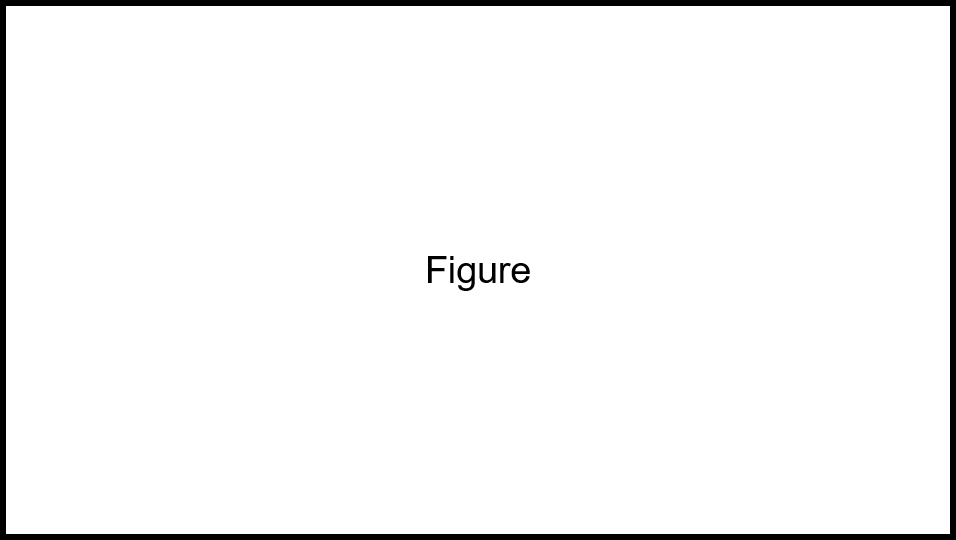
\includegraphics[width=0.7\textwidth]{fig1.png}
    \caption{図のキャプション}
    \label{fig:my_label}
\end{figure}

なお,絵本の挿絵などとは異なり,論文における図はすべて本文中の適切な箇所から参照されているべきである.
その場合,「上図」や「下図」のように位置関係を用いて参照するのではなく,
「図\ref{fig:my_label}」のように番号を用いて参照するのが原則である.

\subsubsection{表の挿入方法}
表は\TeX の table 環境の中で tabular 環境を用いることで作成できる.

\begin{table}[tbhp]
    \caption{表のキャプション}
    \centering
    \begin{tabular}{lcr}
        \hline
        head1 & head2 & head3 \\ 
        \hline\hline
        123 & 456 & 789\\
        \hline
    \end{tabular}
    \label{tab:my_label}
\end{table}

図の場合と同様に,論文における表はすべて本文中の適切な箇所から参照されているべきである.
その場合,「上の表」や「下の表」のように位置関係を参照するのではなく,
「表\ref{tab:my_label}」のように番号を用いて参照するのが原則である.

\section{卒業論文テンプレート(Word)の使い方}

卒業論文をMicrosoft Word (以下単にWordという)により執筆する場合は本学が用意したテンプレートファイルを使用することを推奨するが,本学が用意したテンプレートファイルを使用しない場合は,それと同等のフォーマットとなるように作成すること.また,このテンプレートファイルでは,Wordの使い方のサンプルも含めて,各所で執筆に関する有益な情報を小出しにしているので適宜参照してほしい.ただし,実際の論文では一連の情報は適切に集約すべきであり,小出しにするのは良くない方法であるので留意すること.

\subsection{章立ての設定方法}
このサンプルファイルでは,章,節などの見出しを「スタイル」で設定することで,章節番号が自動的に設定されるとともに,目次にも反映されるようになっている.本文と同様に章見出しなどを入力した後,Homeタブの「スタイル」から,章見出しは「見出し1」,節見出しは「見出し2」,項見出しは「見出し3」を設定することで,体裁が整うはずである.

\subsection{目次の設定方法}
前項で述べた方法に従って,章,節などの見出しに正しく「スタイル」が設定されていれば,
これを用いて目次を自動的に作成することができる.
参考資料タブの「目次」の中に「目次の更新」というボタンがあるので,これを用いればよい.

\subsection{図と表の挿入方法}
この項では図と表の挿入例を示す.

\subsubsection{図の挿入方法}
Wordにおける図の挿入方法には様々な方法がある.各自で確認し,自分の使いやすい方法を用いること.ただし,担当教員から特定の方法の指示があった場合は,指示に従うこと.

なお,絵本の挿絵などとは異なり,論文における図はすべて本文中の適切な箇所から参照されているべきである.その場合,「上図」や「下図」のように位置関係を用いて参照するのではなく,「図1.1」のように番号を用いて参照するのが原則である.


\subsubsection{表の挿入方法}
Wordにおける表の挿入方法には様々な方法がある.各自で確認し,自分の使いやすい方法を用いること.ただし,担当教員から特定の方法の指示があった場合は,指示に従うこと.

図の場合と同様に,論文における表はすべて本文中の適切な箇所から参照されているべきである.その場合,「上の表」や「下の表」のように位置関係を参照するのではなく,「表1.1」のように番号を用いて参照するのが原則である.


 
\chapter{関連研究}	% TODO: 章題を記入.題は任意.
\thispagestyle{plain}   % chapterの直後に必ず指定

%TODO: 章の内容を記入.以下はサンプル.
章のタイトルのあと,各節に入る前に書かれるこの部分のことを「リード文」という.リード文の役割は,論文全体の中でその章が持つ役割を明確にすることである.
リード文は必ずなければならないというものではないが,だいたいの場合はあったほうがよいものである.
たとえばこの章であれば,「この章では,関連研究について述べるとともに,
関連研究と対比させて本研究の位置づけを明確にする.」のような内容を記述する.
なお,関連研究はこのように独立した章にしてもよいし,序論の中に組み込んでもよい.

\section{関連研究に関する節その1}
この節では○○に関する関連研究について述べる.

\subsection{関連研究に関する項その1}
この項では○○に関する関連研究のうち,△△について述べる.

\subsection{関連研究に関する項その2}
この項では○○に関する関連研究のうち,▲▲について述べる.

\section{関連研究に関する節その2}
この節では□□に関する関連研究について述べる.


 
\chapter{提案手法}	% TODO: 章題を記入.題は任意.
\thispagestyle{plain}   % chapterの直後に必ず指定

%TODO: 章の内容を記入.以下はサンプル.
この章では提案手法について述べる.
研究内容に応じ,提案する理論/仮説/モデル/アルゴリズム/システム/方法論/実装などについて説明する.
この部分が論文の主たる部分となる.章のタイトルはサンプルに縛られるものではなく,研究内容に応じて当然変わるものであるし,
章の数も,研究内容に応じて適切に設定すべきである.適切に担当教員からの指導を受けること.
以上を踏まえて,この章では,カレーライスの食べ方について,詳細に説明する.

\section{把持}
まず,スプーンを手に持つ.この際,落とさないようにしっかりと持つことが重要である.

\section{掘削}
スプーンをカレー皿に挿入し,一口で食べられる適量をスプーンに載せる.

\section{運搬}
スプーンをカレー皿から取り出し,口元まで運ぶ.掘削の際に過剰な量をスプーンに載せていると,この段階でスプーンからこぼれ落ちる可能性があるので注意が必要である.

\section{摂食}
口元まで運んだスプーンを口腔内に挿入し,スプーンに載っていたカレーを摂食する.

 
\chapter{実験と評価および考察}	% TODO: 章題を記入.題は任意.
\thispagestyle{plain}   % chapterの直後に必ず指定

%TODO: 章の内容を記入.以下はサンプル.
この章では本研究で行った実験と評価および考察について述べる.
研究内容によっては,考察は独立の章に分けたほうが適切なことも多い.
また,実験と評価と考察で節を分けなければならないというものでもない.
自らの研究内容を論文にまとめるにあたって,最も適切な方法を選択することが重要である.
それはそれとして,この章では,数式の書き方と,参考文献のリスト法
について記述する.
研究分野によっては慣習が異なることがあるので,適切に担当教員からの指導を受けること.
%出典は昨年度までのWordテンプレートである.

\section{数式}
数式は \TeX の数式モードを使うと美しく表記できるので,数式を多く使う論文は \TeX を用いて作成することを推奨する.
一方,Wordにも数式を作成する機能はあり,挿入タブの「記号と特殊文字」の中に「数式」ボタンがあるので,これを用いて作成することができる.
以下に数式が2つ記載されているが,\TeX 版のテンプレートファイルのものは \TeX で作成したものであり,
Word版のテンプレートファイルのものは Word で作成したものである.2つのpdfを見比べると,それぞれの違いがわかるはずである.
\begin{equation} \label{identity_matrix}
I=\begin{pmatrix} 1 & 0 \\ 0 & 1 \end{pmatrix}
\end{equation}
\begin{equation} \label{integral}
\int x^n dx =\frac{1}{n+1} x^{n+1} +C 
\end{equation}
ここで$I$は単位行列,$C$は積分定数を表す.
なお,$I$をIと書いてしまうと,$I$とは別のものと見なされるので注意すること.
数式を参照するときは,(\ref{identity_matrix})のように参照したり,
式(\ref{identity_matrix})のように参照したり,
(\ref{identity_matrix})式のように参照したりとさまざまなルールがあるので,
担当教員の指導に従うこと.
なお \TeX における数式番号の自動参照については,まさにこの部分を記載しているソースコードが参考になるはずである.一方,Wordにおける数式番号の挿入方法および自動参照には様々な方法がある.各自で確認し,自分の使いやすい方法を用いること.ただし,担当教員から特定の方法の指示があった場合は,指示に従うこと.

\section{参考文献}
参考文献の引用方法や記載方法も,分野の慣習により異なることがあるので,担当教員の指導に従うこと.
とくに文献の記載方法は分野や雑誌によって多種多様なフォーマットが用いられているが,
いずれにしても,異種のフォーマットが混在している記載方法は良くない記載方法である.
各所からコピーアンドペーストしたものをまとめると,異種のフォーマットが混在することになりがちなので気をつけること.
たとえば著者名であれば,Yasuhiro Katagiri と Y. Katagiri と Katagiri, Y. が混在しているのは典型的な悪いリストである.
同様に,文献タイトルにおいても,
``How to play and win the Monopoly game.''(文頭と固有名詞のみ大文字)と
``How to Play and Win the Monopoly Game.''(冠詞・前置詞・接続詞以外は大文字)が混在しているのは典型的な悪いリストである.
月の省略形も ``Sep.'' と``Sept.'' が混在しているのは悪いリストである.
こういった点に注意を払うのも論文執筆者の務めである.
各種学会で文献の記載方法をルールとしてまとめているので,適宜参照するとよいと思われるが,いずれにしても担当教員の指導に従うこと.

 
\chapter{結論}	% TODO: 章題を記入.題は任意.
\thispagestyle{plain}   % chapterの直後に必ず指定

%TODO: 章の内容を記入.以下はサンプル.
この章は最終章である.
第1章と最終章は対比がとれていることが望ましい.
具体的には,「序論」ではじめたのなら「結論」で終わり,
「はじめに」ではじめたのなら「おわりに」で終わる.
「緒言」ではじめたのなら「結言」で終わる.

\section{句読点}
日本語の文書で一般に用いられる読点には「、」「,」の2種類があり,
句点には「。」「.」の2種類がある.
情報系では「,.」を用いることが多いが,
どちらを用いるべきかは分野の慣習により異なることがあるので,指導教員の指示に従うこと.
いずれにしても,両者が無秩序に混在しているのは悪い文書である.

\section{まとめ}
論文の執筆法は,研究分野によりさまざまなルールや慣習がある.
また,研究内容に応じ,最適な章立てや叙述の順序なども異なってくる.
このスタイルファイルに書かれている内容はあくまで例にすぎない.
実際に論文を執筆し,提出する際は,担当教員の指導に従うこと.
また,論文の書き方や研究の進め方を指南する書籍やウェブサイトは多数存在するので,
適宜参照すると良い.
この場合も,分野によって論文の書き方や研究の進め方が異なることはあるので,
担当教員の指導を受けることが望ましい.
 
% 以下必要に応じてchapterX.texを作成してinput文を記入

% TODO: 謝辞
\pagestyle{plain}
\chapter*{謝辞}
% TODO: 謝辞を以下に記入

謝辞を記入する.


% TODO: 発表等実績
% \chapter*{発表・採録実績}

% TODO: 発表・採録実績(確定分も含む)を以下の例のように記入

\subsection*{発表等}
\begin{enumerate}
\renewcommand{\labelenumi}{[\arabic{enumi}]}
    \item 情報処理学会 第82回全国大会(2020年3月)
\end{enumerate}


% TODO: 参考文献
% TODO: 参考文献を以下のように記入.

\begin{thebibliography}{99}
 \bibitem{item1}
Reference1
 \bibitem{item2}
Reference2
\end{thebibliography}


% TODO: 付録.必要がなければ削除すること
\appendix
\chapter*{付録}	% TODO: 章題を記入.題は任意.
\thispagestyle{plain}   % chapterの直後に必ず指定

%TODO: 章の内容を記入.以下はサンプル.
プログラムのソースリスト,その他関連資料などを,【必要があれば】載せる.
必要ない場合は,このページごと削除すること.
\TeX の場合は main.tex 内の \yen appendix 以下の2行を削除(またはコメント化)すればよい.
Wordの場合は前のページの「改ページ」以降を削除すればよい.
 

% 図表一覧等自動生成
%\listoffigures
%\thispagestyle{plain}
%\listoftables
%\thispagestyle{plain}


\end{document}
